\chapter{Xây dựng mô hình}
\label{Chapter3}
\section{Tiền xử lý dữ liệu}

Chúng ta nhận thấy rằng trong một số đoạn hội thoại sẽ có những thẻ như file photo, hãy xem qua một ví dụ:\\

\begin{figure*}[htp]
    \centering
    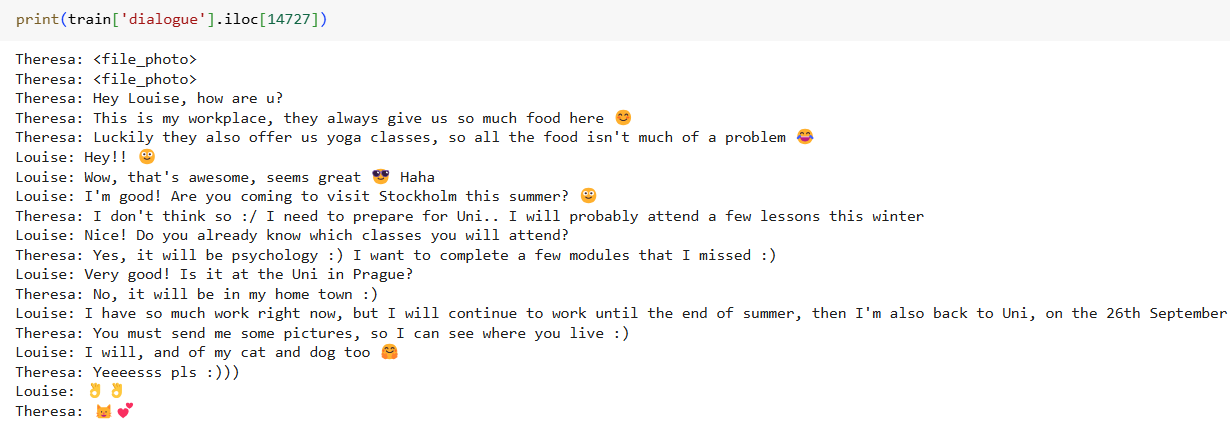
\includegraphics[scale=.6]{images/vd1.png}
    \end{figure*}

Để loại bỏ các thẻ này khỏi văn bản, giúp văn bản trở nên sạch hơn, chúng ta sẽ sử dụng hàm clean-tags được định nghĩa dưới đây:\\

\lstinputlisting[language=Python]{SourceCode/clean_tags.py}


\begin{figure*}[htp]
    \centering
    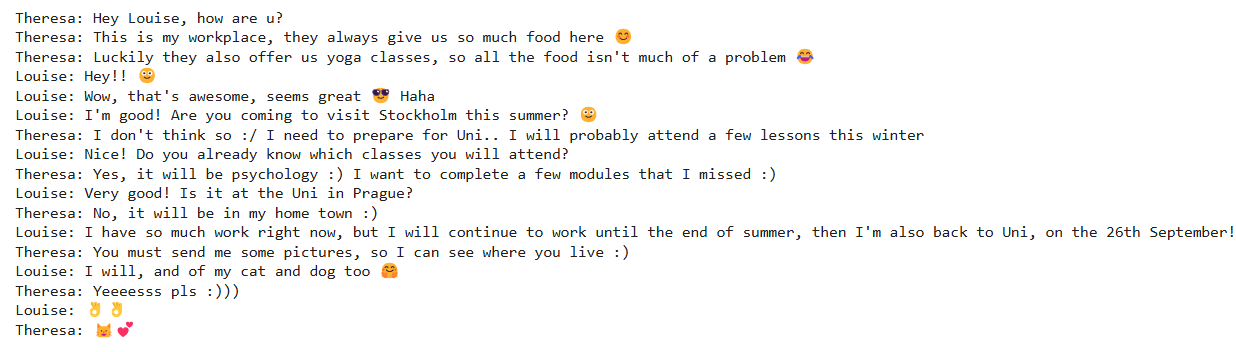
\includegraphics[scale=.6]{images/ketqua.png}
    \end{figure*}

Có thể thấy rằng chúng ta đã loại bỏ thành công các thẻ khỏi văn bản. Bây giờ, chúng ta sẽ định nghĩa hàm clean-df, trong đó sẽ áp dụng hàm clean-tags cho toàn bộ 
các bộ dữ liệu.\\

\lstinputlisting[language=Python]{SourceCode/clean_df.py}

Các thẻ đã được loại bỏ khỏi văn bản. Việc thực hiện quá trình dọn dẹp dữ liệu như vậy là rất có ích để loại bỏ nhiễu - những thông tin không đóng góp đáng kể vào ngữ cảnh tổng thể và có thể làm giảm hiệu suất.

Bây giờ, chúng ta sẽ thực hiện một số bước tiền xử lý cần thiết để chuẩn bị dữ liệu của chúng ta làm đầu vào cho mô hình đã được huấn luyện sẵn và để tinh chỉnh mô hình. Phần lớn những gì chúng ta đang làm ở đây là một phần trong hướng dẫn về Tóm tắt Văn bản được mô tả trong tài liệu của Transformers.

Đầu tiên, chúng ta sẽ sử dụng thư viện Datasets để chuyển các Pandas DataFrame của chúng ta thành Datasets. Điều này sẽ giúp dữ liệu của chúng ta sẵn sàng để xử lý trong toàn bộ hệ sinh thái của Hugging Face.\\

\lstinputlisting[language=Python]{SourceCode/transf.py}

Sau khi chuyển đổi thành công các Pandas DataFrames thành Datasets, chúng ta có thể tiếp tục với quá trình mô hình hóa.\\

\section{Mô hình hóa}
Như chúng ta đã đề cập trước đó, chúng ta sẽ tinh chỉnh một phiên bản của BART đã được huấn luyện trên nhiều bài báo tin tức cho nhiệm vụ tóm tắt văn bản, đó là facebook/bart-large-xsum.
Chúng ta sẽ trình bày ngắn gọn mô hình này bằng cách tải một pipeline tóm tắt với mô hình này để cho bạn thấy cách nó hoạt động trên dữ liệu tin tức.\\

\lstinputlisting[language=Python]{SourceCode/loadbart.py}

Ví dụ, chúng ta sẽ sử dụng bài báo tin tức sau, được xuất bản trên CNN vào ngày 24 tháng 10 năm 2023, với tiêu đề "Bobi, the world's oldest dog ever, died aged 31". Lưu ý rằng đây là một bài báo tin tức hoàn toàn mới mà chúng ta đưa vào mô hình, để có thể xem nó hoạt động như thế nào.\\

\lstinputlisting[language=Python]{SourceCode/new.py}


\begin{figure}[htp]
	\centering
	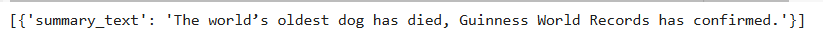
\includegraphics[width=16cm, height=2cm]{images/kq}

\end{figure}

\pagebreak
Bạn có thể quan sát thấy rằng mô hình có thể tạo ra một đoạn văn bản ngắn gọn hơn rất nhiều, chứa đựng thông tin quan trọng nhất từ văn bản đầu vào. Đây là một ví dụ tóm tắt thành công.

Tuy nhiên, mô hình này đã được huấn luyện chủ yếu trên các tập dữ liệu bao gồm nhiều bài báo tin tức từ CNN và Daily Mail, chứ không phải trên nhiều dữ liệu hội thoại. Vì vậy, chúng ta sẽ tiến hành tinh chỉnh nó với SamSum dataset.
    
Bây giờ, chúng ta sẽ tải BartTokenizer và BartForConditionalGeneration sử dụng checkpoint facebook/bart-large-xsum.\\
